\documentclass[12pt,a4paper]{article}
\usepackage{geometry}
\usepackage[numbers]{natbib}
\usepackage{amssymb, amsmath}
\usepackage{graphicx}
\usepackage{grffile}
\graphicspath{{../Figures/}}
\usepackage{gensymb}
\usepackage[font=small]{caption}
\usepackage[utf8]{inputenc}
\usepackage[english]{babel}
\usepackage{fancyhdr}
\usepackage[raggedright]{titlesec}
\usepackage{subcaption}
\usepackage{multirow}
\usepackage{dirtytalk}
\usepackage{framed}
\usepackage[normalem]{ulem}
\usepackage[pdftex,breaklinks]{hyperref}
\hypersetup{
  colorlinks   = true, %Colours links instead of ugly boxes
  urlcolor     = green, %Colour for external hyperlinks
  linkcolor    = blue, %Colour of internal links
  citecolor   = red %Colour of citations
}


\begin{document}
\author{Katrina Ashton}


\pagestyle{fancy}
\fancyhf{}
\rhead{\thepage}
\lhead{u5586882}

\section{What I've done}
\begin{itemize}
\item Worked on registration algorithm: added alignment (not using ROS), applied RANSAC to points
%\item{Added more to the appendices for the final report draft}
\end{itemize}

\section{Parts of report to look at}
\begin{itemize}
\item Nothing since last week
\end{itemize}

\section{Questions}
\begin{itemize}
\item
\end{itemize}

\section{Comments}
\begin{itemize}
\item I talked to Zheyu yesterday, he should be done with the RealSense so I'll pick it up today and work on the pipeline (try to integrate ROS?). I told him I'd try to give it back to him on Monday.
\item The ground truth values are global, w.r.t. to the coordinates defined by a motion capture system (as specified on the dataset website).
\item RANSAC is used as part of the function for finding the Essential Matrix in opencv. But as I didn't do it to the points directly it hasn't been done of Kabsch (I did some thresholding for the distances though).
\item The Essential Matrix finding function gives you a mask of inliers and outliers, so I'm now using this to filter the points for recovering the pose and Kabsch.
\item I added alignment between the RGB and depth images when performing the registration (repeating depth images where necessary), and between the ground truth and registration results during evaluation (repeating registration results where necessary)
\item The feature-matching only method seems to have actually gotten worse.
\item Looking at the matches before and after removing the points with RANSAC, they seem much better but some images still have outliers present. I should try using a higher threshold. 
\item I'm still getting very bad results, might need to do some kind of blur detection to filter bad images. 
\item I should check that the depth images are actually aligned with the RGB images (time stamps and per-pixel. On the website it says they are already aligned per-pixel, but they don't look like it). Maybe make a point cloud and see if it looks sensible?
\item Need to fix up my write-up on finding the Essential Matrix and write a separate section on what the Essential Matrix actually is.
\item I'm currently using rotation matrices within my registration function but storing the trajectory as Quaternions.
\end{itemize}

\begin{figure}[t!]
  \centering
  \begin{subfigure}[t]{\textwidth}
  \centering
    \includegraphics[width=120mm, trim =10mm 30mm 10mm 30mm, clip]{../data/rgbd_dataset_freiburg2_pioneer_slam/matches/1311878194.439904_before.png}
  \caption{Before RANSAC}
  \end{subfigure}
  \\
  \begin{subfigure}[t]{\textwidth}
  \centering
    \includegraphics[width=120mm, trim =10mm 30mm 10mm 30mm, clip]{../data/rgbd_dataset_freiburg2_pioneer_slam/matches/1311878194.439904_after.png}
  \caption{After RANSAC}
  \end{subfigure}
  \caption{Feature matches before and after RANSAC with prob=0.999, threshold=1.0. Note that RANSAC has not removed all outliers}
  \label{f: D415 offset}
\end{figure}

\begin{figure}[t!]
  \centering
  \begin{subfigure}[t]{0.5\textwidth}
  \centering
    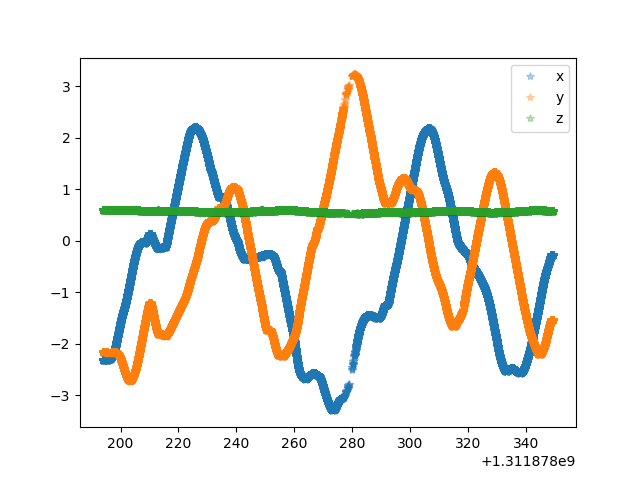
\includegraphics[width=60mm]{../2018-UAV-Registration/basic-reg-saves/trj_gt.png}
  \caption{Position trajectory, ground truth}
  \end{subfigure}%
  ~
  \begin{subfigure}[t]{0.5\textwidth}
  \centering
    \includegraphics[width=60mm]{../2018-UAV-Registration/basic-reg-saves/axis_gt.png}
  \caption{Axis of rotation, ground truth}
  \end{subfigure}
  \\
  \begin{subfigure}[t]{0.5\textwidth}
  \centering
    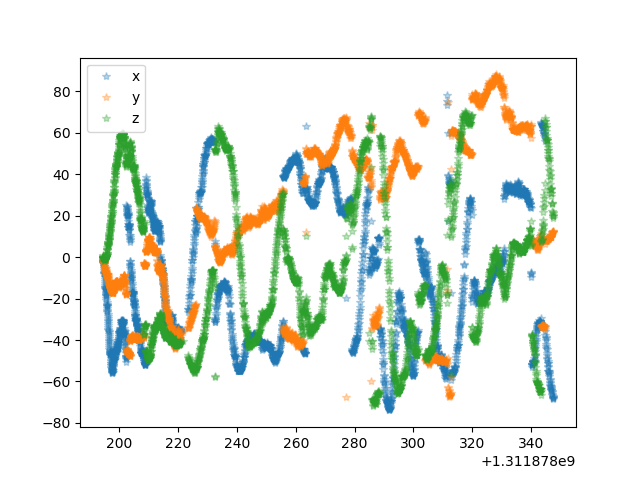
\includegraphics[width=60mm]{../2018-UAV-Registration/basic-reg-saves/trj_rgb.png}
  \caption{Position estimated trajectory for Essential Matrix method}
  \end{subfigure}%
  ~
  \begin{subfigure}[t]{0.5\textwidth}
  \centering
    \includegraphics[width=60mm]{../2018-UAV-Registration/basic-reg-saves/axis_rgb.png}
  \caption{Axis of rotation estimation for Essential Matrix method}
  \end{subfigure}
  \\
  \begin{subfigure}[t]{0.5\textwidth}
  \centering
    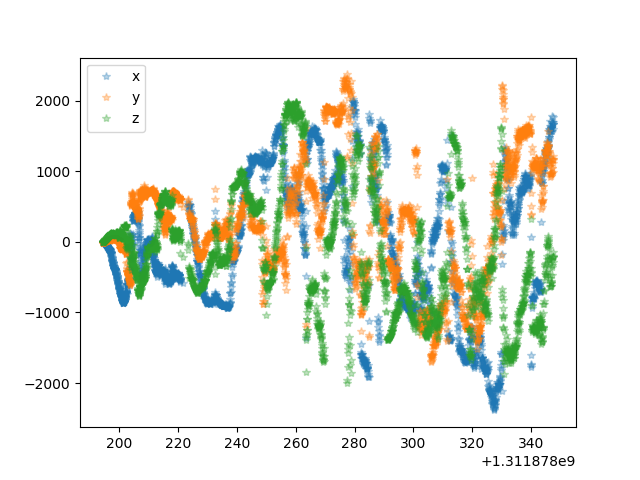
\includegraphics[width=60mm]{../2018-UAV-Registration/basic-reg-saves/trj_d.png}
  \caption{Position estimated trajectory for Kabsch method}
  \end{subfigure}%
  ~
  \begin{subfigure}[t]{0.5\textwidth}
  \centering
    \includegraphics[width=60mm]{../2018-UAV-Registration/basic-reg-saves/axis_d.png}
  \caption{Axis of rotation estimation for Kabsch method}
  \end{subfigure}
  \caption{Trajectory visualizations. Begins at yellow, then goes into green and then blue}
  \label{f: D415 offset}
\end{figure}

\begin{figure}[t!]
  \centering
  \begin{subfigure}[t]{0.5\textwidth}
  \centering
    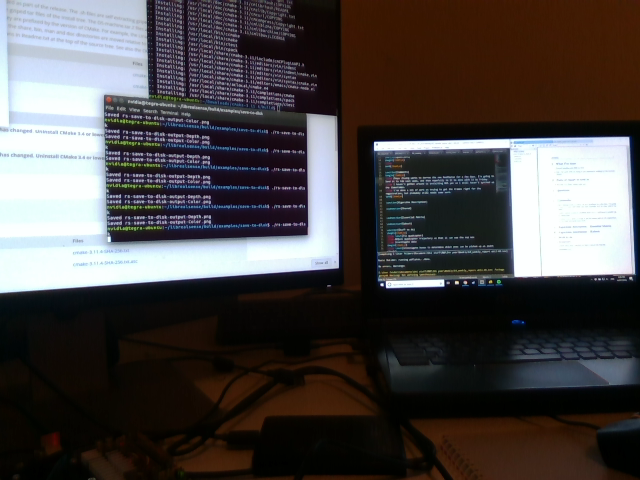
\includegraphics[width=60mm]{camera_tests/rs-save-to-disk-output-Color.png}
  \caption{Colour Image (640 x 480)}
  \end{subfigure}%
  ~
  \begin{subfigure}[t]{0.5\textwidth}
  \centering
    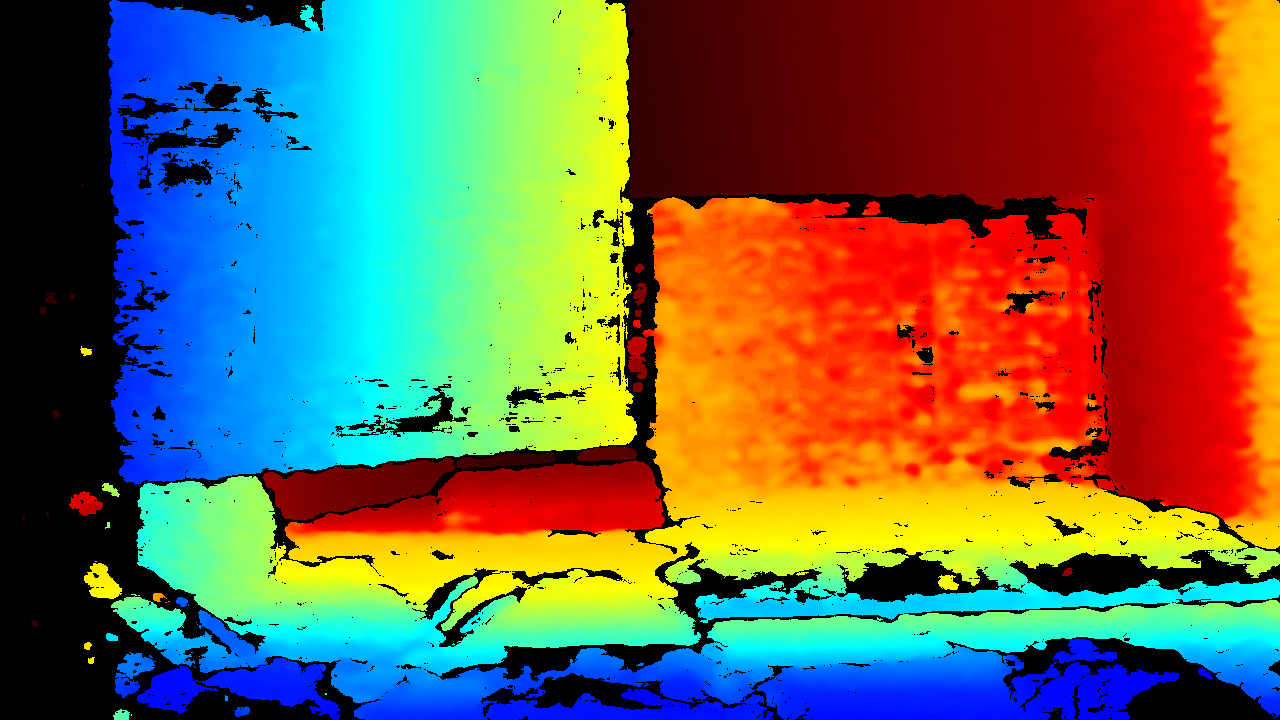
\includegraphics[width=60mm]{camera_tests/rs-save-to-disk-output-Depth.png}
  \caption{Depth Image (1280 x 720)}
  \end{subfigure}
  \caption{Images captured from RealSense RD415, note that the image dimensions are different and the depth image captures more of the scene to the right}
  \label{f: D415 offset}
\end{figure}


\section{Algorithm Description}
\label{sec: algo}

\subsection{Shared}
For each approach, the reconstructed trajectory of the camera is stored in two arrays: one with the x,y and z components of the position, and another with the w, x, z and z components of a Quaternion that gives the orientation. These formats were chosen as it is how the ground truth is stored.
\\\\
The initial position and orientation are initialized as the first values in the ground truth.
\\\\
Next, the frames are looped over. Right now the timestamps are not aligned, so I'm looping over the number of depth images as there are less of them. The following will describe what happens in each loop.
\\\\
The current RGB image and the one from the next timestamp are both loaded. The keypoints of each image are found using SIFT, they are then matched using a brute force method. The matches are then ordered in terms of their distance (i.e. how good a match they are). 
\\\\
The matches are then iterated over, and matches with a distance of less than 180 (found via trial and error) are kept. If there are less than 6 points the Essential Matrix cannot be found, so the loop is restarted with the next frame. If there are more than 6 points, two different methods are used to recover the camera pose: finding the Essential Matrix (see Section \ref{ssec: essential mat}), and aligning matched 3D points using Kabsch (see Section \ref{ssec: kabsch}).

\subsection{Essential Matrix}
\label{ssec: essential mat}
The Essential Matrix $E$ can be found in opencv using matched points and the focal length and principal point of the camera. This is done using Nister's five-point algorithm \cite{nister2003efficient}. Note that in practice more than five points may be required to ensure the estimation is robust and accurate. With more than five points, the fve-point algorithm can be used as a hypothesis generator within a random sample consensus scheme (RANSAC). That is, five point correspondences are chosen at random, then the five-point algorithm is used to estimate the Essential matrix from them, this estimate is a hypothesis. This process is repeated to get a number of hypotheses, which are scored using a robust statistical measure over all points. This gives an overall estimate of the best hypothesis, which can be improved iteratively as more sets of five point correspondences are used. In opencv this process does not necessarily use all possible sets of five point correspondences; it stops once the probability of the hypothesis being correct has reached the specified probability threshold.
\\\\
The algorithm itself uses the fact that a real non-zero $3\times 3$ matrix $E$ is an essential matrix if and only if it satisfies
\[
EE^TE - \frac{1}{2}trace(EE^T)E = 0
\]
There are additional constraints imposed by each point correspondence: $\tilde{q}^t \tilde{E} = 0$ where
\begin{align*}
\tilde{q} &\equiv \begin{bmatrix} q_1q_1' & q_2q_1' & q_3q_1' & q_1q_2' & q_2q_2' & q_3q_2' & q_1q_3' & q_2q_3' & q_3q_3' \end{bmatrix}^T \\
\tilde{E} &\equiv \begin{bmatrix} E_{11} & E_{12} & E_{13} & E_{21} & E_{22} & E_{23} & E_{31} & E_{32} & E_{33} \end{bmatrix}^T 
\end{align*}
The $\tilde{q}^T$ vectors for the five points can then be stacked to get a $5 \times 9$ matrix. Then four vectors $\tilde{X}, \tilde{Y}, \tilde{Z}, \tilde{W}$ that span the right nullspace of this matrix are found (when there are multiple possibilities, the ones corresponding to the smallest singular values are used). These vectors correspond to four $3\times 3$ matrices $X, Y, Z, W$, which can be used to find the Essential Matrix as 
\[
E = xX + yY + zZ + wW
\]
for some scalars $x,y,z,w$, it is assumed $w=1$ as these scalars are only defined up to a common scale factor. This equation can then be inserted into the $9 \times 5$ constraint matrix. This can then be used to find $x,y$ and $z$ (see \cite{nister2003efficient} for details), and thus $E$ can be found from $E = xX + yY + zZ + wW$.
\\\\
Opencv can then be used to recover the relative pose difference of the camera using the above information and the Essential Matrix. The process for doing this is also described in \cite{nister2003efficient}. At least one point is needed to resolve ambiguities by imposing a cheirality constraint (i.e. all scene points should be in front of the cameras).

\subsection{Kabsch}
\label{ssec: kabsch}
Once the matched points have been found, a depth needs to be associated with each one. Currently the pixel with the same indices as the RGB image is taken from the depth image. However upon inspecting the data more closely it seems like the RGB and depth images are not aligned, thus more processing will be necessary to find the corresponding point in the depth image.
\\\\
Once the corresponding depth has been found, a 3D point is defined with the $x$ and $y$ components from the RGB image width and height, respectively and the depth as the $z$ component. As these points are matched, the Kabsch algorithm can be used to align them.
\\\\
However, before this can be done the points need to be converted out of the image frame and into the camera frame. To do this, the following equations are used
\begin{align*}
z^c &= z^i /sf \\
x^c &= (x^i - cx)*z^c / fx \\
y^c &= (y^i - cy)*z^c / fy \\
\end{align*}
Where the superscript indicates the frame ($c$ for camera, $i$ for image), $sf$ is a scaling factor provided by the makers of the dataset, $cx$ and $cy$ are the $x$ and $y$ components of the optical center, and $fx$ and $fy$ are the $x$ and $y$ components of the focal length.
\\\\
Then Kabsch is applied. First, a $P$ and $Q$ matrix are defined, with each row being a point (first column $x$, second $y$, third $z$).The points are then centered, this is done by subtracting from each row in the matrix the centroid of that matrix. (The centroid is the sum of all the elements divided by the number of elements, done separately for each component). The translation is then given by the centroid of $Q$ minus the centroid of $P$.
\\\\
Next, the cross-covariance matrix, $H$, is found:
\[
H = P^T Q
\]
The rotation matrix from $P$ to $Q$ is given by 
\[
R = (H^TH)^{1/2}H^{-1}
\]
To actually calculate this, the singular value decomposition (SVD) is used:
\begin{align*}
H &= USV^T \\
d &= \text{det}(VU^T) \\
R &= V \begin{bmatrix} 1 & 0 & 0 \\ 0 & 1 & 0 \\ 0 & 0 & d \end{bmatrix} U^T
\end{align*}

\subsection{Updating global trajectory}
After the pose is acquired (as a translation and rotation matrix), the global trajectory needs to be updated. We have pose in the camera frame, so we can update the trajectories as follows:
\begin{align*}
Q_{m}^{g,n} &= Q_{m}^{g,n-1} * Q_{m}^{c,n} \\
P_{m}^{g,n} &= P_{m}^{g,n-1} + Q_{m}^{g,n-1}(P_{m}^{c,n})
\end{align*}

\noindent
Where $Q$ are the orientations (in quaternions), and $P$ are the positions. The subscript is for the method used for registration ($rgb$ for using only the RGB images via the Essential Matrix, and $d$ for also using the depth images via Kabsch). The superscript starts with the frame the measurement is in ($g$ for global, $c$ for camera, $i$ for image) and then gives the timestep the measurement is for (where $n$ is the current timestep).
\\\\
Note that the first position is not rotated, as it is already in the global frame. The second position is rotated, as it is in the camera frame (this is the translation found by registration). This position is rotated by the global rotation from the last timestep, as it is in the camera frame (i.e. with respect to the camera orientation at the end of the last timestep).


\section{Stuff to do}
\begin{itemize}
\item Adjust quadcopter trajectory so that it can see the top box
\item Write acquisition code for D415
\item Investigate data
\begin{itemize}
\item \sout{Investigate boxes to determine which ones can be picked up as point clouds}
\item \sout{Investigate RealSense cameras, compare the two cameras and using them on TX1/TX2 or Windows/Ubuntu}
\end{itemize}
\item Investigate registration algorithm
\begin{itemize}
\item Generate 3D object in MATLAB that I can get points from from various camera poses (may also need to get RGB and depth images if we're going with that approach?)
\item Apply registration algorithm to generated point clouds (ground truth known) -- without noise first, then add noise. Get error in true and estimated translation and rotation.
\end{itemize}
\item Try registration on external dataset
\begin{itemize}
\item Feature-only method (Essential Matrix)
\item Feature and depth method (Kabsch)
\item Install ROS and use it to align timestamps
\item Ensure that every pose is given with respect to the appropriate frame (ground truth is given in global frame, so each registered pose should be stored in global frame)
\item Incorporate IMU data
\end{itemize}
\item Reading
\begin{itemize}
\item \sout{Incorporating RGB and depth images -- feature matching (papers you sent me)}
\item Write up summary of main points (parts of the algorithm, choices with advantages/disadvantages)
\item See if more recent papers have made advancements
\end{itemize}
\end{itemize}

\bibliographystyle{abbrvnat}
\bibliography{../Report/ENGN4217}

\end{document}